 %% Copyright (C) 2021 by
 %%   Robert L. Read <read.robert@gmail.com>, Megan Cadena <megancad@gmail.com>

 %% This program is free software: you can redistribute it and/or modify
 %% it under the terms of the GNU General Public License as published by
 %% the Free Software Foundation, either version 3 of the License, or
 %% (at your option) any later version.

 %% This program is distributed in the hope that it will be useful,
 %% but WITHOUT ANY WARRANTY; without even the implied warranty of
 %% MERCHANTABILITY or FITNESS FOR A PARTICULAR PURPOSE.  See the
 %% GNU General Public License for more details.

 %% You should have received a copy of the GNU General Public License
 %% along with this program.  If not, see <http://www.gnu.org/licenses/>.

\documentclass{article}
\usepackage[backend=biber]{biblatex}
\addbibresource{softrobotmath.bib}
\usepackage{hyperref}
\usepackage{amsmath}
\usepackage{amssymb}
\usepackage{mathtools}
\usepackage{draftwatermark}
\usepackage{listings}

\usepackage{flexisym}
\usepackage{breqn}
\breqnsetup{breakdepth={1}}

\SetWatermarkText{DRAFT}
\SetWatermarkScale{6}
\SetWatermarkLightness{0.95}

\title{Three Inflatable Spheres as a Theoretical Basis for a Parallel Manipulator}

\author{Robert L. Read
  \thanks{read.robert@gmail.com}
  email: \href{mailto:read.robert@gmail.com}{read.robert@gmail.com}\\
Megan Cadena
  \thanks{megancad@gmail.com}
  email: \href{mailto:megancad@gmail.com}{megancad@gmail.com}
  }


\begin{document}
\maketitle

\begin{abstract}
  A Stewart Platform\cite{wiki:stewart} is a fundamental mechanism for varying the angle
  between two objects.
  A soft Stewart Platform can be made of two discs and
  three inflatable spheres.
  Soft robots are meant to deform under force, but it is useful to have
  a closed-form description of a plane in contact with three spheres of changing size.
  This papers gives closed-form expressions for the plane in contact with
  three adjacent spheres from known radii, and closed-form expressions for
  the much harder inverse problem of finding the radii to match a plane inclination.
  An interactive,
  browser-based web page that dynamically solves the problem\cite{softrobotcalc}
  using JavaScript implementations of this math.
\end{abstract}


\section{Introduction}

A parallel manipulator varies the angle between two planes.
The best known parallel manipulator is
a Stewart Platform\cite{wiki:stewart} which as 6 degrees or freedom.
Having a soft parallel manipulator analogous to a Stewart Platform would allow soft,
gentle positioning,
and might be particularly valuable {\it in vivo}\cite{white2018soft} or in some space applications\cite{glassner2020soft}.
Varying angular displacement is a composable building block of more complicated systems, such as tentacles.

One theoretical way to build such a manipulator is to have three enlargeable spheres sandwiched between two planes
and constrained to always be in contact with each other.
As these spheres are enlarged, perhaps by pneumatically inflating them changing
their size, the top plane changes its orientation relative to the bottom plane.
This creates 3 degrees of rotational freedom
(ignoring the slight translation the spheres are capable of by consistently enlarging),
which is slightly more constrained than the 6DOF Stewart Platform.
In 1881, the problem of computing the plane tangent to three spheres was
set as an exercise in a textbook, {\em Practical Solid Geometry}\cite{payne1881},
but not solved.

The forward problem is given three radii,
to determine the orientation of the top plane.
The inverse problem is much harder: given a desired orientation and the radius of one
sphere, find the radius of the other two spheres that achieves it.
This paper gives closed-form expressions of both
the forward and inverse problem of three inflatable spheres as a parallel manipulator as pure solid geometry.

Additionally, we have created an online, interactive, browser based real-time simulation\cite{softrobotcalc} that implements
the math in this paper in JavaScript, both verifying it and making it easy to reuse.
All of the code is released under the GNU Public License\cite{gplv3}.

Soft robotics presume to operate under some deforming forces, so in any deformable robot the precise mathematics
of positioning must always be corrected by a control system with feedback on the position.
Nonetheless, having a closed-form expression of both the inverse and forward problem allow
an initial Jacobian to be computed effortlessly, which is likely to assist any soft robotic control algorithm.

\section{The Center Plane}

As kinematicists,
our interest is in the slope of the plane of the tops of these spheres
as if they were resting on a fixed-frame such as a table. Then by inflating or deflating spheres,
we would be able to control the direction of the top plane or platform.

Choosing the coordinate system of the $XZ$ plane through the center of the spheres greatly
simplifies the derivations, because the center of the spheres always form tangent circles
in this plane. Call this plane the {\em center plane.}
Following computer graphics convention, we think of the $Y$ dimension as vertical and a
right-handed set of axes.
The position of $A$ is fixed at the origin, $B$ is constrained to the $x$-axis touching $A$, and
$C$ is constrained to the positive $xz$-plane. The center of these circles in the $xz$ plane can be
calculated from the radii independent of the tilt they induce.
In this coordinate system, the $y$-coordinate of the center of all spheres is $0$.
Furthermore, a cone tangent to two spheres has its axis and apex in the $xz$-plane.
The projection of all three spheres into this plane produces three touching circles.
We seek an expression for the normal of the plane of the tops of these spheres as a function
purely of the three radii. Call this plane the {\em top plane}.
We can imagine the spheres resting on a fixed surface called the {\em bottom plane}.
The tilt of the top and bottom plane relative to the center of the spheres
is alway a mirror image of each other across the coordinate $XZ$-plane.


Define extrinsic Euler angles $\theta$ to be the rotation about the $Z$-axis and then $\gamma$ to
be the rotation about the $X$-axis.
The tilt of the top plane relative
to the bottom plane is given by the $zx$ extrinsic Euler angles $(2\theta, 2\gamma)$.\footnote{Is this really true?
We should be able to verify this with a JavaScript program.}

Because there is a plane through any three points and we have three spheres, we can construct the plane through
the center of these points.
The projection of the edges of the spheres onto this plane form three touching circles.

\begin{figure}
     \centering
     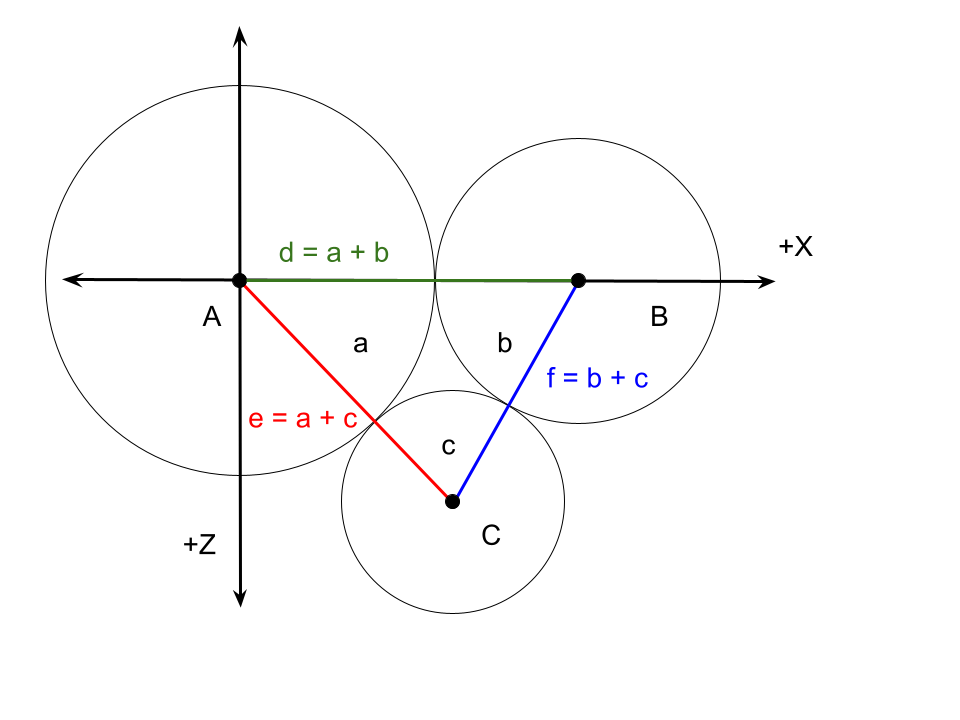
\includegraphics[width=0.8\textwidth]{figures/ThreeTouchingPlanarCircles.png}
     \caption{Three Touching Circles}
  \label{fig:Tangent}
\end{figure}

To solve this problem most conveniently, we place the first circle at the origin, and the second circle
on the positive $x$-axis, with the circles intersecting at the origin.
The third circle is place in the positive $z$ direction touching both other circles.

We seek a formula for the coordinates of the third circle in terms of three input radii $a,b,c$.

Because the distance between adjacent circles is the sum of their radii, define:
\begin{align}
  d  &= a + b \\
  e  &= a + c \\
  f  &= b + c \\
\end{align}

Considering Fig. \ref{fig:Tangent}, varying the radius $c$ without constraint will cause
the center of the circle $C$ to move, as shown by the dotted circles,
describing a gentle curve depicted by the dashed curve which at very large $c$ is perpendicular to a
line tangent to both $A$ and $B$, indicated by the dotted line.
By considering the desired tilt of the top plane,
a particular point on this curve is chosen.

\subsection{The half-angle of a cone enveloping two tangent spheres}

The apex half-angle $\psi$ of a cone which envelopes (by being tangent to) two tangent
spheres of radii $r,s$, is purely a function of $r$ and $s$.
Luckily, to develop a formula for $\psi$, we can treat the problem as a two-dimensional problem,
as shown in Fig. \ref{fig:conehalf}


\begin{figure}
     \centering
     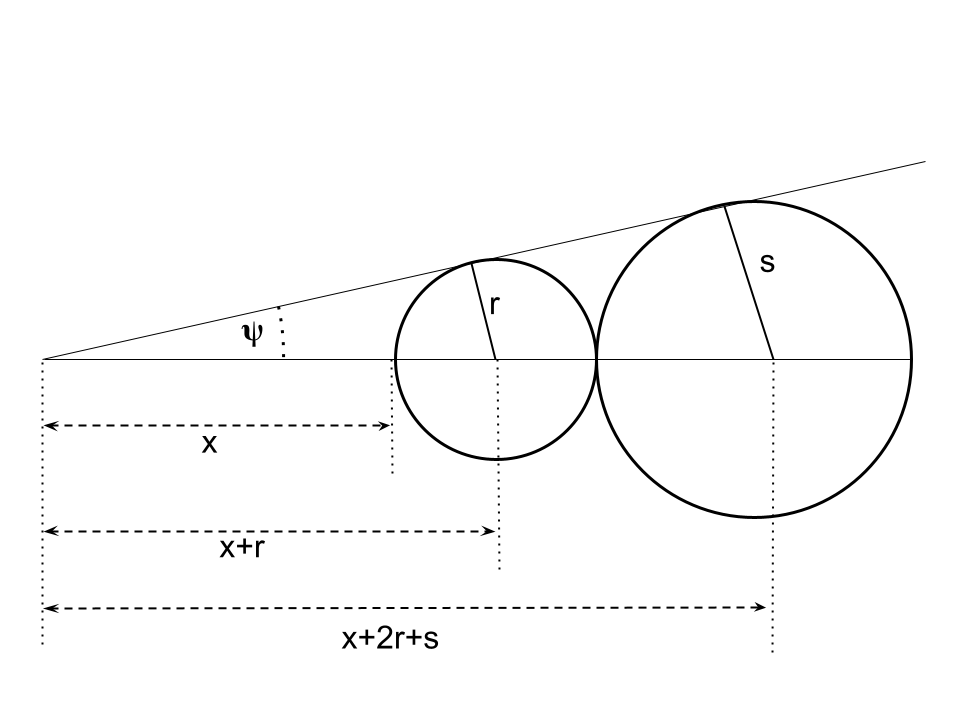
\includegraphics[width=0.8\textwidth]{figures/HalfAngleOfConeTangenttoTwoTangentSpheres.png}
     \caption{Half-angle of Cone Tangent to Two Tangent Spheres}
  \label{fig:conehalf}
\end{figure}

Noting the lengths of the hypotenuses as shown in the figure, we
can calculate $x$ in terms of $r$ and $s$:

\begin{align}
  \sin{\psi} &= \frac{r}{x + r} \\
  \sin{\psi} &= \frac{s}{x + 2r + s} \\
  \frac{r}{x + r} &= \frac{s}{x + 2r + s} \\
  s(x + r) &= r(x + 2r + s) \\
  x &= \frac{2r^2}{s - r}
\end{align}
We can then eliminate $x$:
\begin{align}
  \sin{\psi} &= \frac{r}{x + r} \\
  \sin{\psi} &= \frac{r}{\frac{2r^2}{s - r} + r} \\
    \sin{\psi} &= \frac{1}{\frac{2r}{s - r} + 1} \\
      \sin{\psi} &= \frac{s-r}{2r + s - r} \\
    \sin{\psi} &= \frac{s-r}{r + s} \\
 \psi &= \arcsin{\frac{s - r}{s + r}}
\end{align}
where $r < s$ without loss of generality. Note that when $r = s$
there is a special case,
the cone tangent to both is degenerate (that is, a cylinder, or a cone of
$\psi = 0$ apex angle.)


\section{The Euler Anglers from the Radii}

\subsection{Finding the Point C}

Given $a,b$ and $c$, we seek the angles $\theta$ and $\gamma$ representing
the Euler anglers of rotation around the $Z$ axis ($\theta$), and then the $X$ axis ($\gamma$).

We seek the  point $C$ first.
Call the angle $\angle ABC = \epsilon$, since the opposite side
is labeled $e$.
The cosine law to compute the angle $\epsilon$:

\begin{align}
  \epsilon  &= \arccos{\frac{d^2 + f^2 - e^2}{2fd}}
\end{align}

It is clear that once $\epsilon$ has been calculated
we can calculate $C_z$:\footnote{We use the common convention that $C_x, C_y, and C_z$ represent the $x$, $y$ and $z$
coordinate of the point or vector $C$.}

\begin{align}
 C_z  &= f\sin{\epsilon}
\end{align}
Noting that $B_x = d = a + b$,
\begin{align}
  C_x   &= d - \cos{\epsilon}
\end{align}


\subsection{The Apex Line}

\begin{figure}
     \centering
     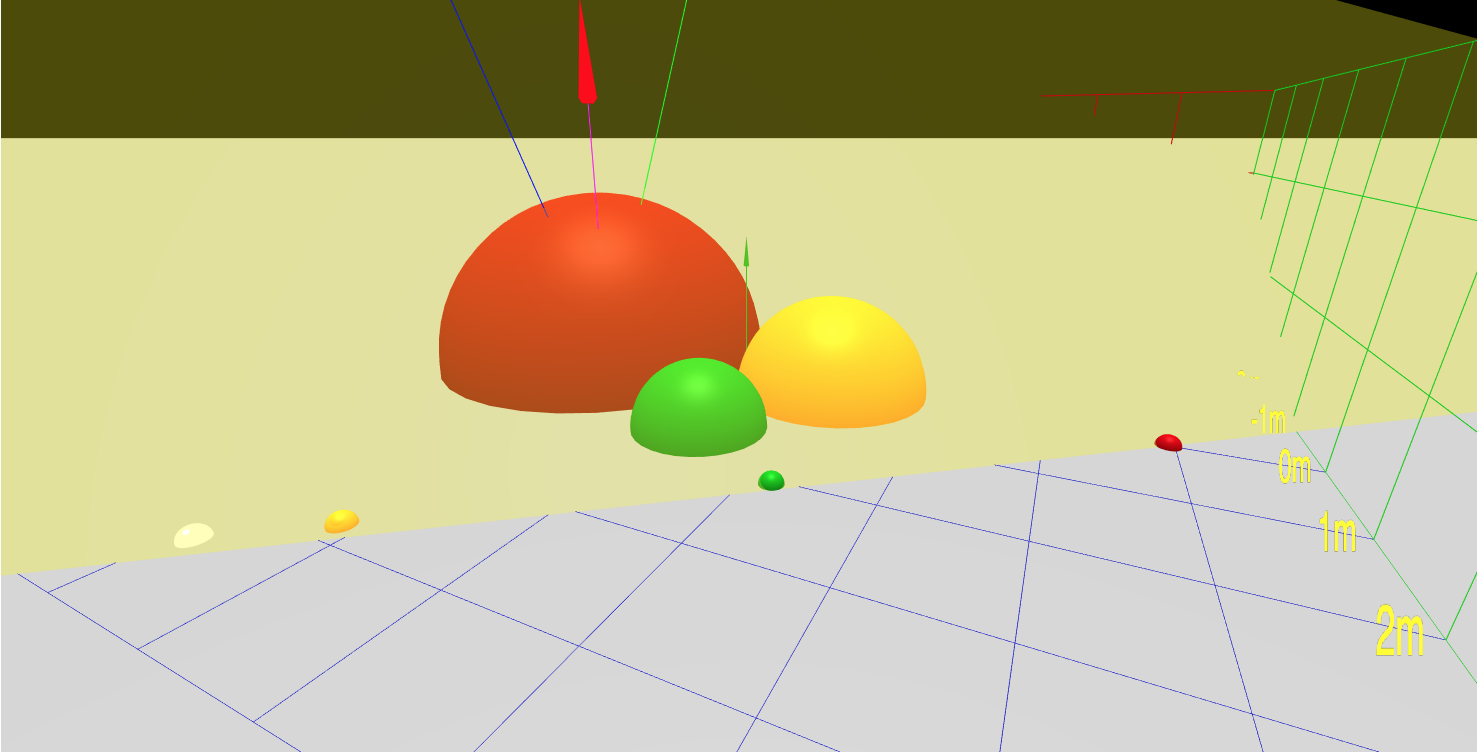
\includegraphics[width=0.99\textwidth]{figures/StandardThreeSphereDiagram.png}
     \caption{Three Touching Spheres}
  \label{fig:fixed}
\end{figure}

The problem of finding the planes tangent to three touching spheres
is given as an exercise in an advanced textbook on solid geometry from 1881\cite{payne1881} which does not give a solution,
but it gives a hint: to consider the cones enveloping
three spheres taken two at a time.

Taking two adjacent spheres defines a cone tangent to both spheres whose apex is in the $XZ$ plane.
Call the apex of the $AB$ cone $U$, the $AC$ cone $V$, and the $BC$ cone $W$.

It is a beautiful fact that the the apices $U,V$ and $W$ are collinear
on the {\em apex line} which is in the $XZ$ plane, depicted in both Figure \ref{fig:fixed}
or Figure \ref{fig:rotation}.
Finally, the top and bottom planes
intersect at this line, because those planes are tangent to the three cones.

Observe that this plane is tangent to all three cones.
Observe that the $AB$ cone intersects
the $A$ sphere in a circle on the surface of the $A$ perpendicular to and centered on the $X$ axis.

The apex half-angle $\psi$ of a cone which envelopes (by being tangent to) two tangent
spheres of radii $r,s$, is:
\begin{align}
 \psi_{abs} &= \arcsin{\frac{s - r}{s + r}}
\end{align}
where $r < s$ without loss of generality. Note that when $r = s$
there is a special case,
the cone tangent to both is degenerate (that is, a cylinder, or a cone of
$\psi = 0$ apex angle.)

Let $\theta$ be the rotation of the ground plane (the $XZ$ plane in this system) need to make
it rest on the $A$ and $B$ spheres and intersect the $AB$ cone.
Because we use $\theta$ as a rotation angle, it must be signed, and is
negative if $a > b$.
\begin{align}
  \theta &= \begin{cases}
    \theta, & \text{ if $a > b$, } \\
    -\theta, & \text{  otherwise}
\end{cases} \label{eq:theta} \\
\end{align}

\subsection{Computing $\gamma$}

Note that in this paper, like THREE.js and many computer graphics systems,
we use a right-handed coordinate system and describe angles of rotation as
positive when counter-clockwise looking from a positive axis as the origin.

\begin{figure}
     \centering
     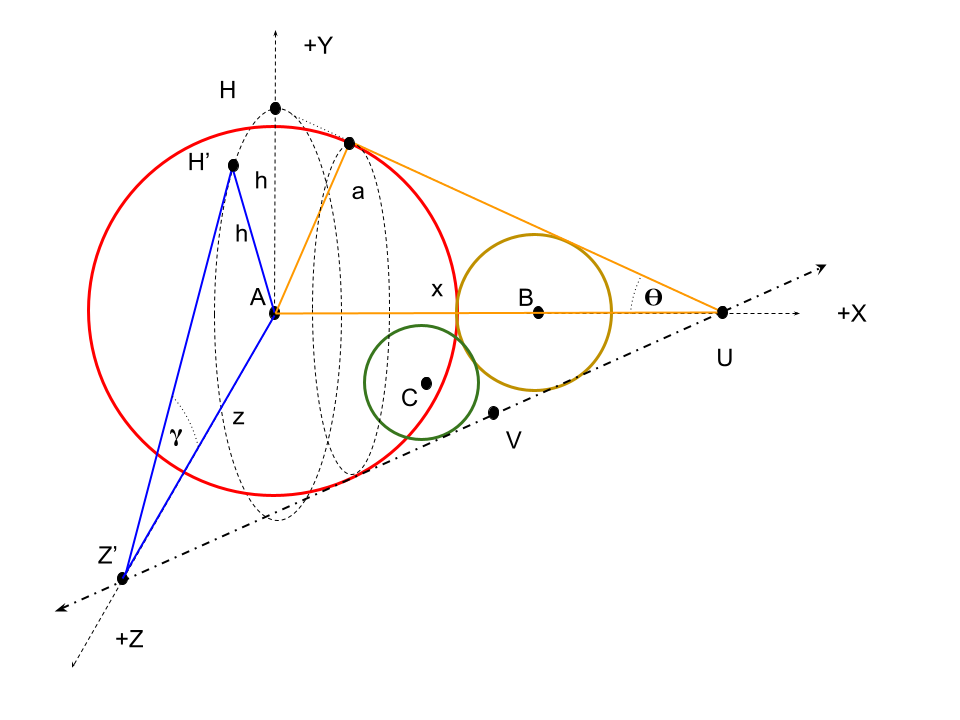
\includegraphics[width=0.9\textwidth]{figures/RotationMathII.png}
     \caption{Rotation Math}
  \label{fig:rotation}
\end{figure}

In our main view (see Fig. \ref{fig:rotation}) and in the initial view
of our software, thus has a positive $\gamma$ and negative $\theta$, when $a > b$ and $a > c$.

In order to compute $\gamma$, we seek to form a triangle in the $YZ$ plane.
Because Euler angles are performed in a certain order, it is necessary to imagine
the ground plane after it has been rotated by $\theta$ but before it has been rotated by $\gamma$.
Call this the ``Z-rotated'' plane.



After a rotation of $\theta$ about the $Z$ axis, the Z-rotated plane intersects the $X$ axis
at a point $U = [U_x,0,0]$, the apex of the AB cone:
\begin{align}
  U_x = \frac{a}{\sin{(-\theta)}}
\end{align}

The $y$ coordinate of the point $H$ where where the top plane intersects
the $Y$ axis is:
\begin{align}
  H_y &= U_x \tan{\theta}
\end{align}

Any rotation about the $X$ axis of the Z-rotated plane (and $H$) will keep that
point in the $YZ$ plane and a distance $ h = H_y$ from the origin.

Call the intersection
of the $Z$-axis apex line with apex line $Z'$, and let $z = Z_z$.
Then $\gamma$ is the angle we need to rotate the plane already rotated by $\theta$ so that it intersects with the
$Z$-axis at $Z'$.
Points $U$ and $V$ represent the apices of the apices of the cones tangent to $A$ and $B$, $A$ and $C$, respectively.
The apex of the $BC$ cone, $W$, is also on the apex line but not used in our calculations.

The point $V$ is computable as the apex of the $AC$ cone:
\begin{align}
  \phi &= \arcsin{\frac{a - c}{a + c}} \\
  V &= A + (C-A) \frac{b}{\sin{\phi}} \\
  V &= C (\frac{b(a+c)}{a-c}) \\
\end{align}

The $z$ coordinate of the point $Z'$ can be calculated from
$Z$ intercept
fact that it is collinear with $U$ and $V$, which has a slope
in the $XZ$ plane of $\frac{V_z}{U_x-V_x}$:
\begin{align}
  z&= \begin{cases}
    V_z, & \text{ if $a = b$ } \\
    \frac{V_z U_x}{U_x - V_x}, & \text{ if  $a \neq b$}
  \end{cases}
  \label{eq:zprime} \\
\end{align}

The line $Z'H'$ is tangent to a circle of radius $h$ around the point $A$
in the $YZ$ plane, so $\angle Z'H'A$ is a right angle.
The point $H'$ is in the top plane by definition and $Z'$ is in the top plane
because it is on the apex line.
The hypotenuse of the $\triangle Z'H'A$ is the line $AZ'$ on the $Z$ axis of
length $z$, and the angle $\gamma = \angle AZ'H$ has an opposite side of length $h$,
so:
\begin{align}
  \gamma &= \arcsin{\frac{h}{z}} \label{eq:gamma}
\end{align}

Equations \ref{eq:theta} and \ref{eq:gamma} give the Euler angles
as a rotation $\theta$ about the $Z$ axis followed by a rotation $\gamma$ about the $X$ axis
for the tangent plane as a function of the three radii $a,b,c$

\section{The Inverse Problem}

To build a theoretic robotic platform by controlling the radii of the
spheres by inflating and deflating them, we wish to solve the inverse
problem. That is, given input $\theta$ and $\gamma$ as desired Euler
angles, we want to compute $a,b,c$ which achieve these angles.

Since these are smooth functions, the problem could be solved
easily by a Newton-Raphson style solver based on \ref{eq:theta} and \ref{eq:gamma}.
However, a closed-form solution is always superior, and allows derivatives,
and hence Jacobians, to be expressed symbolically as closed-form solutions.

The radius $b$ can be computed directly from $\theta$
because of our choice of coordinates.
By considering to proportionality of the similar triangles formed
by the contacts points of sphere $A$ and $B$ and their centers with $U_x$ in the $XY$ plane,
we obtain:
\begin{align}
  U_x &= \frac{a}{\sin{\theta}} \\
  b &= \frac{(U_x - a)\sin{\theta}}{\sin{\theta}+1}
\end{align}

\newcommand{\abs}[1]{ \left\lvert#1\right\rvert}

Given the plane defined by a known radius $a$, $\theta$ and $\gamma$,
the point $C$ is constrained by asserting that the perpendicular
distance to this plane of $C$ is $c$.
Additionally, in the central plane we have two other constraints,
that $C$ is placed so that it touches the circle centered on $A$ and
the circle centered on $B$.

Then we do not know the point $C$ but know the distance $a+c$ from
the point $A$ (the origin) and the distance $b+c$ from the known
point $B$. These two constraints can be generated from the Pythagorean Theorem and can be expressed:
\begin{align}
a + c &= \sqrt{C_x^2 + C_z ^2} \label{eq:a_constraint}\\
b + c &= \sqrt{(a+b-C_x)^2 + C_z^2} \label{eq:b_constraint}
\end{align}

If we were to plot the point $C$ as $c$ increases, we
would find a gentle curve moving away from the intersection
of the circle $A$ and $B$, curling in the direction of the smaller of $A$ or $B$.
An additional constraint will
designate a point on this curve.
This gives us three equations, which
should be more than enough to solve for the point $C$.

Let $H = [0, H_y,0]$.

Let $N$ be the normal to the plane (pointing up in our diagram
when $ a >= b >= c $.)

\begin{align}
\overrightarrow{N} &= \overrightarrow{Z' - U}  \times \overrightarrow{Z' - H}
\end{align}

Since we have the normal of the plane and three points ($U,Z,H_y$) in the plane,
computing the distance from the point $C$ to the plane has a simple
formula.
We'll use the point $U = [Ux, 0, 0]$ as our main point.
In our situation, because the sphere $A$ is at the origin,
the equation of the top plane  is
$ \overrightarrow{N} \cdot \overrightarrow{U} = a$.
\begin{align}
a &= \frac{N \cdot U}{N_y} \\
c &= \frac{\abs{N \cdot P - a}}{\abs{N}} \\
c &= \frac{\abs{C_x  N_x  + C_z  N_z - a}}{1} \label{eq:c_constraint}
\end{align}

By substituting \ref{eq:c_constraint} into equations
\ref{eq:a_constraint} and \ref{eq:b_constraint},
we obtain:
\begin{align}
  a + \abs{C_x N_x + C_z N_z - a} &= \sqrt{C_x^2 + C_z^2} \\
  b + \abs{C_x N_x + C_z N_z - a} &= \sqrt{(a+b-C_x)^2 + C_z^2}
\end{align}

If the interior expression $C_x N_x + C_z N_z - a$ is positive,
then upon solving the system we find only imaginary solutions.

So assuming it is negative, we obtain:
\begin{align}
  2a + -C_x N_x + -C_z N_z  &= \sqrt{C_x^2 + C_z ^2} \\
  2b + -C_x N_x + -C_z N_z  &= \sqrt{(a+b-C_x)^2 + C_z^2}
\end{align}

This is a system of two nonlinear equations with unknowns $C_x$ and $C_z$.
Solving this system is beyond symbolic manipulating capacities of the authors,
but not Mathematica.
However, Mathematica expends half a page expressing the answer
in its raw form.

Furthermore, there are actually two solutions, corresponding
to the two sides of the $AB$ line which the circle $C$ could be
on and satisfy these constraints.
We have selected the solution that place $C$ in the positive $Z$
direction conformant to our problem set-up.

However, by introducing new variables to represent repeated
portions of this long expression, the expressions be
made tractable and easily programmed by computer.

\begin{align}
M &= (a + b + a N_x - b N_x)^2 - 4 a b N_z^2 \\
L &= a (a + b + a N_x - b N_x) - b (a + b) N_z^2 \\
G &= -a^2 (a - b)^2 b N_z^2 \\
H &= 2 a (-1 + N_x) - b ((-1 + N_x)^2 + N_z^2) \\
F &= \sqrt{G H} \\
K &= 4 a^2 b^2 N_z^2 + 2 a^3 b (-3 + N_x) N_z^2 \\
J &= b^3 (-1 + N_x) N_z^2 \\
C_{x0} &= \frac{2 (F + a L)}{M} \\
C_{z0} &= \frac{K + (2 b F (-1 + N_x) -
  2 a (F (1 + N_x) + b^3 (-1 + N_x) N_z^2))}
{(a -  b) M N_z} \\
C_{x1} &= \frac{-2 F + 2 a L}{M} \\
  C_{z1} &= \frac{K - (2 b F (-1 + N_x) -
  2 a (F (1 + N_x) + b^3 (-1 + N_x) N_z^2))}
  {(a - b) M N_z}
\end{align}

One solution ($(C_{x0},C_{z0})$ or $(C_{x1},C_{z1})$) will be on the
positive side of the $X$ axis, but which one is highly dependent
on the input variables, so both are computed and the positive $z$
value selected.

The variable $c$ can be computed from $a$, $C_x$ and $C_z$
form Eqn. \ref{eq:a_constraint}.

This math can be found in the JavaScript which is licensed
under the GPL\cite{gplv3} at our website\cite{softrobotcalc}.

\section{Special Cases of the Inverse Problem}

When both $\theta = 0$ and $\gamma = 0$, then $c = b = a$.

\subsection{Special case when $\gamma$ is $0$ }

In the above math when $\gamma = 0$, then $N_z$ is zero,
creating a division by zero.
In this case we can use the proportionality of similar
triangles to assert:
\begin{align}
  a &= c + \frac{a C_x}{U_x}
\end{align}
Combined with our previous equations
Eqn. \ref{eq:a_constraint} and Eqn. \ref{eq:b_constraint} in the plane
relating $C_x$ and $C_z$ to $c$,
we obtain the following equation:
\begin{align}
c & = \frac{a (a + b) (a - U_x)}{a^2 - a b + a U_x + b U_x}
\end{align}


\subsection{Special case when $\theta$ is $0$ }

When $\theta = 0$, the point $U$ is at infinity or
cannot be found. In this case $b = a$.
In this case the sphere $C$ is symmetrically
positioned in contact with $A$ and $B$ because
they have the same radius; therefore $C_x = a$ and:
\begin{align}
(a + c)^2 &= a^2 + C_z^2
\end{align}

In this case,
\begin{align}
Z' &= \frac{a}{\sin{\gamma}}
\end{align}

Projecting out the $X$ dimension and forming
similar triangles in the $YZ$ plane, we find that
\begin{align}
  c &= \frac{a( Z' -C_z )}{Z'} \label{eqn:cthetazero}
\end{align}

Asking Mathematica to solve these two non-linear equations, we obtain,
after again discarding the solution producing negative $z$ values:
\begin{align}
 C_z &=  \frac{2 a^2 Z' - \sqrt{a^4 (Z')^2 + 3 a^2 (Z')^4}}{a^2 - (Z')^2},
\end{align}
which allows us to obtain obtain $c$ from \ref{eqn:cthetazero}.

\section{Future Work and Relation to Robotics}

Our formulation of the problem with the center of the spheres in the $XZ$
plane has allowed us to obtain a closed-form solution to both the forward
and inverse problem.

A Stewart Platform could be constructed of three inflatable spheres.
However, our formulation is inconvenient for that problem, because
in practice you would know the bottom plane, and not the central plane,
as you vary the diameters of the spheres through inflation or deflation.
The angle between the top and bottom plane will be approximately but not
exactly twice the angles that we have computed here.

We attempted to solve this problem by reformulating the problem in terms
of a coordinate system based on fixed bottom plane, but
the formulae became intractably long even with the help of Mathematica.
However, as a completely deterministic solid geometry system, there
must be a closed-form solution, that perhaps mathematicians of greater
skill or diligence can find.
For example, it might be fruitful to reformulate the problem purely
in terms of the normal of the top plane as a linear algebra problem rather than
considering Euler angles.

Even if one had such a solution, it would be of limited value
to robotocists because the inflation or deflation of spheres in
a macroscopic physically constructible Stewart platform would
be ``soft'', and would deform under external pressure. The solutions
presented here would likely have value only as approximate or initial
solutions.

We conjecture there may be situations in chemistry or astronomy
beyond our ability to identify
in which tangent spheres remain ideal spheres and these closed-form expressions
would remain be accurate.

\section{Conclusion}

Closed-form expressions of the problem of finding a plane resting on
three spheres in contact have been given, and the inverse problem
of finding the radii of three spheres necessary to support a plane
on threes spheres in contact has been solved.
The expressions are in the coordinate system of the the center
of the threes spheres, which may be a significant limitation for some
applications.

An interactive, browser-based solution that allows real-time manipulation
of the mathematical system in both the forward and inverse directions
using sliders has been given\cite{softrobotcalc}. The greatest value of this work
may be the demonstrating the attractiveness of the solution.
The existing of the apex line, which is so visually apparent and pleasing,
may not be completely obvious upon first consideration.

\printbibliography


\end{document}
